% Options for packages loaded elsewhere
% Options for packages loaded elsewhere
\PassOptionsToPackage{unicode}{hyperref}
\PassOptionsToPackage{hyphens}{url}
%
\documentclass[
]{book}
\usepackage{xcolor}
\usepackage{amsmath,amssymb}
\setcounter{secnumdepth}{-\maxdimen} % remove section numbering
\usepackage{iftex}
\ifPDFTeX
  \usepackage[T1]{fontenc}
  \usepackage[utf8]{inputenc}
  \usepackage{textcomp} % provide euro and other symbols
\else % if luatex or xetex
  \usepackage{unicode-math} % this also loads fontspec
  \defaultfontfeatures{Scale=MatchLowercase}
  \defaultfontfeatures[\rmfamily]{Ligatures=TeX,Scale=1}
\fi
\usepackage{lmodern}
\ifPDFTeX\else
  % xetex/luatex font selection
\fi
% Use upquote if available, for straight quotes in verbatim environments
\IfFileExists{upquote.sty}{\usepackage{upquote}}{}
\IfFileExists{microtype.sty}{% use microtype if available
  \usepackage[]{microtype}
  \UseMicrotypeSet[protrusion]{basicmath} % disable protrusion for tt fonts
}{}
\makeatletter
\@ifundefined{KOMAClassName}{% if non-KOMA class
  \IfFileExists{parskip.sty}{%
    \usepackage{parskip}
  }{% else
    \setlength{\parindent}{0pt}
    \setlength{\parskip}{6pt plus 2pt minus 1pt}}
}{% if KOMA class
  \KOMAoptions{parskip=half}}
\makeatother
% Make \paragraph and \subparagraph free-standing
\makeatletter
\ifx\paragraph\undefined\else
  \let\oldparagraph\paragraph
  \renewcommand{\paragraph}{
    \@ifstar
      \xxxParagraphStar
      \xxxParagraphNoStar
  }
  \newcommand{\xxxParagraphStar}[1]{\oldparagraph*{#1}\mbox{}}
  \newcommand{\xxxParagraphNoStar}[1]{\oldparagraph{#1}\mbox{}}
\fi
\ifx\subparagraph\undefined\else
  \let\oldsubparagraph\subparagraph
  \renewcommand{\subparagraph}{
    \@ifstar
      \xxxSubParagraphStar
      \xxxSubParagraphNoStar
  }
  \newcommand{\xxxSubParagraphStar}[1]{\oldsubparagraph*{#1}\mbox{}}
  \newcommand{\xxxSubParagraphNoStar}[1]{\oldsubparagraph{#1}\mbox{}}
\fi
\makeatother

\usepackage{color}
\usepackage{fancyvrb}
\newcommand{\VerbBar}{|}
\newcommand{\VERB}{\Verb[commandchars=\\\{\}]}
\DefineVerbatimEnvironment{Highlighting}{Verbatim}{commandchars=\\\{\}}
% Add ',fontsize=\small' for more characters per line
\usepackage{framed}
\definecolor{shadecolor}{RGB}{241,243,245}
\newenvironment{Shaded}{\begin{snugshade}}{\end{snugshade}}
\newcommand{\AlertTok}[1]{\textcolor[rgb]{0.68,0.00,0.00}{#1}}
\newcommand{\AnnotationTok}[1]{\textcolor[rgb]{0.37,0.37,0.37}{#1}}
\newcommand{\AttributeTok}[1]{\textcolor[rgb]{0.40,0.45,0.13}{#1}}
\newcommand{\BaseNTok}[1]{\textcolor[rgb]{0.68,0.00,0.00}{#1}}
\newcommand{\BuiltInTok}[1]{\textcolor[rgb]{0.00,0.23,0.31}{#1}}
\newcommand{\CharTok}[1]{\textcolor[rgb]{0.13,0.47,0.30}{#1}}
\newcommand{\CommentTok}[1]{\textcolor[rgb]{0.37,0.37,0.37}{#1}}
\newcommand{\CommentVarTok}[1]{\textcolor[rgb]{0.37,0.37,0.37}{\textit{#1}}}
\newcommand{\ConstantTok}[1]{\textcolor[rgb]{0.56,0.35,0.01}{#1}}
\newcommand{\ControlFlowTok}[1]{\textcolor[rgb]{0.00,0.23,0.31}{\textbf{#1}}}
\newcommand{\DataTypeTok}[1]{\textcolor[rgb]{0.68,0.00,0.00}{#1}}
\newcommand{\DecValTok}[1]{\textcolor[rgb]{0.68,0.00,0.00}{#1}}
\newcommand{\DocumentationTok}[1]{\textcolor[rgb]{0.37,0.37,0.37}{\textit{#1}}}
\newcommand{\ErrorTok}[1]{\textcolor[rgb]{0.68,0.00,0.00}{#1}}
\newcommand{\ExtensionTok}[1]{\textcolor[rgb]{0.00,0.23,0.31}{#1}}
\newcommand{\FloatTok}[1]{\textcolor[rgb]{0.68,0.00,0.00}{#1}}
\newcommand{\FunctionTok}[1]{\textcolor[rgb]{0.28,0.35,0.67}{#1}}
\newcommand{\ImportTok}[1]{\textcolor[rgb]{0.00,0.46,0.62}{#1}}
\newcommand{\InformationTok}[1]{\textcolor[rgb]{0.37,0.37,0.37}{#1}}
\newcommand{\KeywordTok}[1]{\textcolor[rgb]{0.00,0.23,0.31}{\textbf{#1}}}
\newcommand{\NormalTok}[1]{\textcolor[rgb]{0.00,0.23,0.31}{#1}}
\newcommand{\OperatorTok}[1]{\textcolor[rgb]{0.37,0.37,0.37}{#1}}
\newcommand{\OtherTok}[1]{\textcolor[rgb]{0.00,0.23,0.31}{#1}}
\newcommand{\PreprocessorTok}[1]{\textcolor[rgb]{0.68,0.00,0.00}{#1}}
\newcommand{\RegionMarkerTok}[1]{\textcolor[rgb]{0.00,0.23,0.31}{#1}}
\newcommand{\SpecialCharTok}[1]{\textcolor[rgb]{0.37,0.37,0.37}{#1}}
\newcommand{\SpecialStringTok}[1]{\textcolor[rgb]{0.13,0.47,0.30}{#1}}
\newcommand{\StringTok}[1]{\textcolor[rgb]{0.13,0.47,0.30}{#1}}
\newcommand{\VariableTok}[1]{\textcolor[rgb]{0.07,0.07,0.07}{#1}}
\newcommand{\VerbatimStringTok}[1]{\textcolor[rgb]{0.13,0.47,0.30}{#1}}
\newcommand{\WarningTok}[1]{\textcolor[rgb]{0.37,0.37,0.37}{\textit{#1}}}

\usepackage{longtable,booktabs,array}
\usepackage{calc} % for calculating minipage widths
% Correct order of tables after \paragraph or \subparagraph
\usepackage{etoolbox}
\makeatletter
\patchcmd\longtable{\par}{\if@noskipsec\mbox{}\fi\par}{}{}
\makeatother
% Allow footnotes in longtable head/foot
\IfFileExists{footnotehyper.sty}{\usepackage{footnotehyper}}{\usepackage{footnote}}
\makesavenoteenv{longtable}
\usepackage{graphicx}
\makeatletter
\newsavebox\pandoc@box
\newcommand*\pandocbounded[1]{% scales image to fit in text height/width
  \sbox\pandoc@box{#1}%
  \Gscale@div\@tempa{\textheight}{\dimexpr\ht\pandoc@box+\dp\pandoc@box\relax}%
  \Gscale@div\@tempb{\linewidth}{\wd\pandoc@box}%
  \ifdim\@tempb\p@<\@tempa\p@\let\@tempa\@tempb\fi% select the smaller of both
  \ifdim\@tempa\p@<\p@\scalebox{\@tempa}{\usebox\pandoc@box}%
  \else\usebox{\pandoc@box}%
  \fi%
}
% Set default figure placement to htbp
\def\fps@figure{htbp}
\makeatother





\setlength{\emergencystretch}{3em} % prevent overfull lines

\providecommand{\tightlist}{%
  \setlength{\itemsep}{0pt}\setlength{\parskip}{0pt}}



 


\makeatletter
\@ifpackageloaded{tcolorbox}{}{\usepackage[skins,breakable]{tcolorbox}}
\@ifpackageloaded{fontawesome5}{}{\usepackage{fontawesome5}}
\definecolor{quarto-callout-color}{HTML}{909090}
\definecolor{quarto-callout-note-color}{HTML}{0758E5}
\definecolor{quarto-callout-important-color}{HTML}{CC1914}
\definecolor{quarto-callout-warning-color}{HTML}{EB9113}
\definecolor{quarto-callout-tip-color}{HTML}{00A047}
\definecolor{quarto-callout-caution-color}{HTML}{FC5300}
\definecolor{quarto-callout-color-frame}{HTML}{acacac}
\definecolor{quarto-callout-note-color-frame}{HTML}{4582ec}
\definecolor{quarto-callout-important-color-frame}{HTML}{d9534f}
\definecolor{quarto-callout-warning-color-frame}{HTML}{f0ad4e}
\definecolor{quarto-callout-tip-color-frame}{HTML}{02b875}
\definecolor{quarto-callout-caution-color-frame}{HTML}{fd7e14}
\makeatother
\makeatletter
\@ifpackageloaded{caption}{}{\usepackage{caption}}
\AtBeginDocument{%
\ifdefined\contentsname
  \renewcommand*\contentsname{Table of contents}
\else
  \newcommand\contentsname{Table of contents}
\fi
\ifdefined\listfigurename
  \renewcommand*\listfigurename{List of Figures}
\else
  \newcommand\listfigurename{List of Figures}
\fi
\ifdefined\listtablename
  \renewcommand*\listtablename{List of Tables}
\else
  \newcommand\listtablename{List of Tables}
\fi
\ifdefined\figurename
  \renewcommand*\figurename{Figure}
\else
  \newcommand\figurename{Figure}
\fi
\ifdefined\tablename
  \renewcommand*\tablename{Table}
\else
  \newcommand\tablename{Table}
\fi
}
\@ifpackageloaded{float}{}{\usepackage{float}}
\floatstyle{ruled}
\@ifundefined{c@chapter}{\newfloat{codelisting}{h}{lop}}{\newfloat{codelisting}{h}{lop}[chapter]}
\floatname{codelisting}{Listing}
\newcommand*\listoflistings{\listof{codelisting}{List of Listings}}
\makeatother
\makeatletter
\makeatother
\makeatletter
\@ifpackageloaded{caption}{}{\usepackage{caption}}
\@ifpackageloaded{subcaption}{}{\usepackage{subcaption}}
\makeatother
\usepackage{bookmark}
\IfFileExists{xurl.sty}{\usepackage{xurl}}{} % add URL line breaks if available
\urlstyle{same}
\hypersetup{
  hidelinks,
  pdfcreator={LaTeX via pandoc}}


\author{}
\date{}
\begin{document}
\frontmatter

\renewcommand*\contentsname{Table of contents}
{
\setcounter{tocdepth}{2}
\tableofcontents
}

\mainmatter
title: ``Spatial Data in R'' format: html editor: visual ---

The \textbf{natural world is fundamentally spatial}. No organism exists
in isolation; every ecological interaction occurs within a specific
environmental context. Scientific observations gain meaning only when
viewed within their spatial and temporal frame. Organisms are subject to
the environmental conditions of their specific place and time. Whether
prey is consumed and transformed through digestion or a leaf decomposes
and returns to the soil, both processes follow fundamental pathways of
pools and fluxes within the spatial and temporal fabric of life.

\begin{figure}[H]

{\centering \includegraphics[width=5.20833in,height=\textheight,keepaspectratio]{images/predator_prey_spatial.gif}

}

\caption{Animated illustration of predator--prey movements across an
environmental gradient, showing how ecological interactions unfold in
space and time.}

\end{figure}%

\textbf{Spatial data} form the foundation of \textbf{geographical
analysis} and \textbf{ecological modeling}. In \textbf{R}, spatial data
are typically managed in two primary formats: \textbf{vector} and
\textbf{raster}.

Recognizing this perspective is essential in environmental science.
Understanding nature's patterns requires data that are organized with
space and time in mind. Fortunately, modern data science in R offers an
excellent toolkit for mapping these relationships and reminding us that
even data, like organisms, thrive best in the right environment.

Beyond data structure, it is increasingly recognized that ecological
observations must be interpreted within an appropriate
\textbf{spatiotemporal context}. Species responses depend not only on
local environmental conditions, but also on \textbf{spatial patterns},
temporal dynamics, and \textbf{scale-dependent processes}. Ignoring
these dimensions can obscure ecological signals or lead to misleading
inferences about species--environment relationships.

Adopting \textbf{tidy data principles} helps structure ecological data
in ways that make relationships between observations, space, and time
explicit. This not only supports more efficient and reproducible
analysis, but also encourages \textbf{conceptual clarity}, enabling
environmental scientists and practitioners to think carefully about what
constitutes an observation, what variables describe it, and how they are
interrelated. Such practices bridge ecological theory with modern data
science workflows, enabling transparent model building, integration
across datasets, and robust generalization of ecological insights.
Ultimately, developing a general understanding of spatial data---and how
it fits within broader data science concepts---is not a technical
luxury, but a conceptual necessity. It strengthens one's ability to
formulate better ecological questions, design meaningful analyses, and
translate data into insight about environmental change, biodiversity
patterns, and ecosystem processes.

\subsubsection{Vector data: Representing discrete
features}\label{vector-data-representing-discrete-features}

\textbf{Vector data} are used to represent \textbf{discrete spatial
features} --- objects with clear boundaries --- such as:

\begin{itemize}
\tightlist
\item
  Tree or animal locations\\
\item
  Roads or rivers\\
\item
  Country or habitat boundaries
\end{itemize}

Vector features are commonly represented in three geometries:

\begin{itemize}
\item
  \textbf{Points}: Individual locations defined by coordinate pairs
  (e.g., species occurrences, weather stations).
\item
  \textbf{Lines}: Linear features such as roads, rivers, or migration
  paths, represented by sequences of connected points.
\item
  \textbf{Polygons}: Closed shapes that define areas like lakes, forest
  patches, or administrative zones.
\end{itemize}

Each vector feature can also include \textbf{associated attributes},
stored in a data table linked to the geometry.\\
These might include:

\begin{itemize}
\tightlist
\item
  species\_name
\item
  survey\_date
\item
  population\_count
\end{itemize}

\subsubsection{Raster Data: Representing Continuous Spatial
Variables}\label{raster-data-representing-continuous-spatial-variables}

\textbf{Raster data} represent \textbf{continuous spatial phenomena} ---
variables that vary smoothly across space --- such as:

\begin{itemize}
\tightlist
\item
  Elevation
\item
  Temperature
\item
  Vegetation indices (e.g., NDVI)
\end{itemize}

A raster is composed of a \textbf{grid of cells} (also called
\emph{pixels}), where \textbf{each cell holds a single value} --- either
\textbf{numeric} (e.g., temperature) or \textbf{categorical} (e.g., land
cover class).

\begin{center}\rule{0.5\linewidth}{0.5pt}\end{center}

\subsubsection{Structure of raster data}\label{structure-of-raster-data}

Unlike vector data, \textbf{raster datasets do not store coordinates for
each cell}. Instead, they rely on:

\begin{itemize}
\tightlist
\item
  \textbf{Spatial extent} -- the geographic boundaries covered by the
  raster\\
\item
  \textbf{Resolution} -- the size of each cell (e.g., 25m x 25m)\\
\item
  \textbf{Origin} -- typically the top-left corner, which anchors the
  raster in space
\end{itemize}

These three components allow computational software like \texttt{R} to
calculate the position of every cell efficiently.

\begin{tcolorbox}[enhanced jigsaw, left=2mm, bottomtitle=1mm, colframe=quarto-callout-tip-color-frame, title=\textcolor{quarto-callout-tip-color}{\faLightbulb}\hspace{0.5em}{Raster and pixels}, breakable, coltitle=black, leftrule=.75mm, bottomrule=.15mm, arc=.35mm, toprule=.15mm, colback=white, toptitle=1mm, rightrule=.15mm, titlerule=0mm, opacityback=0, colbacktitle=quarto-callout-tip-color!10!white, opacitybacktitle=0.6]

Just like digital images, \textbf{raster datasets} can vary in
\textbf{resolution}, which directly affects both \textbf{spatial detail}
and \textbf{file size}.

Higher resolution means finer detail but larger file size, while lower
resolution may be faster to process but less precise.

\end{tcolorbox}

\begin{center}\rule{0.5\linewidth}{0.5pt}\end{center}

\paragraph{Why it matters}\label{why-it-matters}

Understanding the differences, structures, and strengths of both vector
and raster data is essential for:

\begin{itemize}
\tightlist
\item
  Spatial analysis
\item
  Species distribution modeling
\item
  Working with geographic information systems (GIS) in \texttt{R}
\end{itemize}

Throughout this workshop, we'll be using a number of GIS-focused
packages in R. If any of these are not already installed on your system,
you can install them using:

\begin{Shaded}
\begin{Highlighting}[]
\FunctionTok{install.packages}\NormalTok{(}\StringTok{"package\_name"}\NormalTok{, }\AttributeTok{dependencies =} \ConstantTok{TRUE}\NormalTok{)}
\end{Highlighting}
\end{Shaded}

To work with spatial vector and raster data, we'll use the
\texttt{terra} package (for more information, see
\url{https://rspatial.org/index.html}).

If you haven't installed it yet, you can run the following command in
your R console (skip this step if it's already installed):

\begin{Shaded}
\begin{Highlighting}[]
\FunctionTok{install.packages}\NormalTok{(}\StringTok{"terra"}\NormalTok{, }\AttributeTok{dependencies =} \ConstantTok{TRUE}\NormalTok{)}
\end{Highlighting}
\end{Shaded}

Once installed, load the package:

\begin{Shaded}
\begin{Highlighting}[]
 \FunctionTok{library}\NormalTok{(terra)}
\end{Highlighting}
\end{Shaded}

\section{1. Vector data in R - getting
started}\label{vector-data-in-r---getting-started}

Vector data are at the core of spatial data analysis in ecology and
environmental science. In \texttt{R}, vector data are typically managed
using the \textbf{\texttt{terra}} or \textbf{\texttt{sf}} packages, both
of which support reading, manipulating, and visualizing point, line, and
polygon data.

The \texttt{terra} package (which we use in this workshop) handles
spatial vector and raster data in an efficient, modern, and consistent
way.

\begin{center}\rule{0.5\linewidth}{0.5pt}\end{center}

\section{1.1 Points in space}\label{points-in-space}

\subsection{What are spatial points?}\label{what-are-spatial-points}

Points are the simplest vector data geometry and are used to represent
\textbf{individual locations} in space, such as:

\begin{itemize}
\tightlist
\item
  Species occurrence records\\
\item
  Weather stations\\
\item
  Field survey sites\\
\item
  GPS locations
\end{itemize}

Each point is defined by a \textbf{coordinate pair}, typically in
latitude/longitude (geographic) or projected coordinates (e.g., UTM).

\begin{center}\rule{0.5\linewidth}{0.5pt}\end{center}

\subsection{\texorpdfstring{Creating points in \texttt{R} with
\texttt{terra}}{Creating points in R with terra}}\label{creating-points-in-r-with-terra}

You can create spatial points manually using \texttt{vect()} from the
\texttt{terra} package:

\begin{Shaded}
\begin{Highlighting}[]
\FunctionTok{library}\NormalTok{(terra)}

\CommentTok{\# Define coordinates as a matrix for multiple cities (longitude, latitude)}
\NormalTok{coords }\OtherTok{\textless{}{-}} \FunctionTok{matrix}\NormalTok{(}\FunctionTok{c}\NormalTok{(}
  \SpecialCharTok{{-}}\FloatTok{1.2577}\NormalTok{, }\FloatTok{51.7520}\NormalTok{,   }\CommentTok{\# Oxford}
  \FloatTok{12.4964}\NormalTok{, }\FloatTok{41.9028}\NormalTok{,   }\CommentTok{\# Rome}
  \SpecialCharTok{{-}}\FloatTok{3.9440}\NormalTok{, }\FloatTok{51.6214}\NormalTok{,   }\CommentTok{\# Swansea}
   \FloatTok{8.6821}\NormalTok{, }\FloatTok{50.1109}\NormalTok{,   }\CommentTok{\# Frankfurt}
   \FloatTok{8.5417}\NormalTok{, }\FloatTok{47.3769}\NormalTok{,   }\CommentTok{\# Zurich}
   \FloatTok{2.3522}\NormalTok{, }\FloatTok{48.8566}    \CommentTok{\# Paris}
\NormalTok{), }\AttributeTok{ncol =} \DecValTok{2}\NormalTok{, }\AttributeTok{byrow =} \ConstantTok{TRUE}\NormalTok{)}

\NormalTok{city\_name }\OtherTok{\textless{}{-}} \FunctionTok{c}\NormalTok{(}\StringTok{"Oxford"}\NormalTok{, }\StringTok{"Rome"}\NormalTok{, }\StringTok{"Swansea"}\NormalTok{, }\StringTok{"Frankfurt"}\NormalTok{, }\StringTok{"Zurich"}\NormalTok{, }\StringTok{"Paris"}\NormalTok{)}

\CommentTok{\# Create spatial vector of points (longitude, latitude)}
\NormalTok{points }\OtherTok{\textless{}{-}}\NormalTok{ terra}\SpecialCharTok{::}\FunctionTok{vect}\NormalTok{(coords, }\AttributeTok{type =} \StringTok{"points"}\NormalTok{, }\AttributeTok{crs =} \StringTok{"EPSG:4326"}\NormalTok{)}
\NormalTok{points}\SpecialCharTok{$}\NormalTok{city }\OtherTok{\textless{}{-}}\NormalTok{ city\_name}

\CommentTok{\# Get the extent of the points and expand it by 10\% (for plotting)}
\NormalTok{ext }\OtherTok{\textless{}{-}} \FunctionTok{ext}\NormalTok{(points)}
\NormalTok{x\_range }\OtherTok{\textless{}{-}}\NormalTok{ ext[}\DecValTok{1}\SpecialCharTok{:}\DecValTok{2}\NormalTok{]}
\NormalTok{y\_range }\OtherTok{\textless{}{-}}\NormalTok{ ext[}\DecValTok{3}\SpecialCharTok{:}\DecValTok{4}\NormalTok{]}

\NormalTok{x\_margin }\OtherTok{\textless{}{-}} \FunctionTok{diff}\NormalTok{(x\_range) }\SpecialCharTok{*} \FloatTok{0.1}
\NormalTok{y\_margin }\OtherTok{\textless{}{-}} \FunctionTok{diff}\NormalTok{(y\_range) }\SpecialCharTok{*} \FloatTok{0.1}

\NormalTok{x\_ext }\OtherTok{\textless{}{-}} \FunctionTok{c}\NormalTok{(x\_range[}\DecValTok{1}\NormalTok{] }\SpecialCharTok{{-}}\NormalTok{ x\_margin, x\_range[}\DecValTok{2}\NormalTok{] }\SpecialCharTok{+}\NormalTok{ x\_margin)}
\NormalTok{y\_ext }\OtherTok{\textless{}{-}} \FunctionTok{c}\NormalTok{(y\_range[}\DecValTok{1}\NormalTok{] }\SpecialCharTok{{-}}\NormalTok{ y\_margin, y\_range[}\DecValTok{2}\NormalTok{] }\SpecialCharTok{+}\NormalTok{ y\_margin)}

\CommentTok{\# Plot the points with expanded plot extent}
\FunctionTok{plot}\NormalTok{(points, }\AttributeTok{col =} \StringTok{"blue"}\NormalTok{, }\AttributeTok{pch =} \DecValTok{16}\NormalTok{, }\AttributeTok{xlim =}\NormalTok{ x\_ext, }\AttributeTok{ylim =}\NormalTok{ y\_ext)}
\FunctionTok{text}\NormalTok{(points, }\AttributeTok{labels =}\NormalTok{ points}\SpecialCharTok{$}\NormalTok{city, }\AttributeTok{pos =} \DecValTok{4}\NormalTok{, }\AttributeTok{cex =} \FloatTok{0.8}\NormalTok{, }\AttributeTok{col =} \StringTok{"darkblue"}\NormalTok{)}
\end{Highlighting}
\end{Shaded}

\pandocbounded{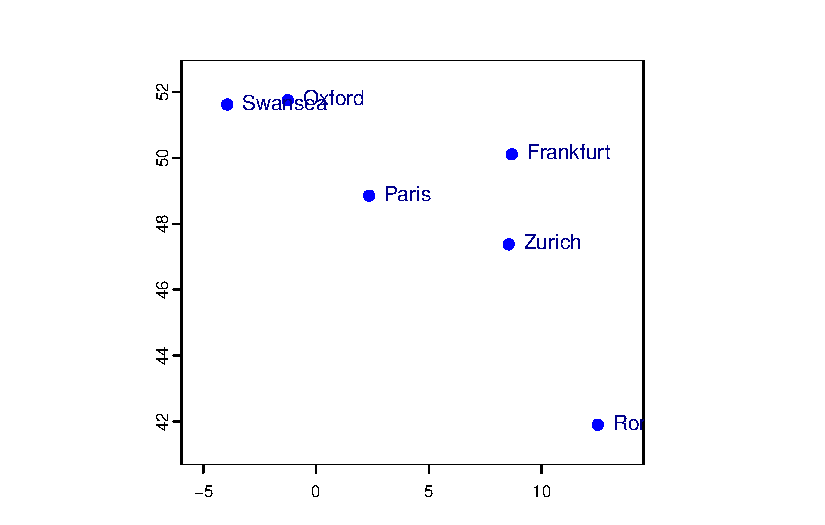
\includegraphics[keepaspectratio]{page_SDM.2_SpatialDataR_files/figure-pdf/unnamed-chunk-4-1.pdf}}

\begin{Shaded}
\begin{Highlighting}[]
\CommentTok{\# Check out the object}
\FunctionTok{class}\NormalTok{(points)}
\end{Highlighting}
\end{Shaded}

\begin{verbatim}
[1] "SpatVector"
attr(,"package")
[1] "terra"
\end{verbatim}

This example creates spatial points for Oxford, Rome, Swansea,
Frankfurt, Zurich, and Paris, using their geographic coordinates
(longitude, latitude), and displays them as blue dots.

\subsubsection{Coordinate reference systems
(CRS)}\label{coordinate-reference-systems-crs}

Every spatial object must have an associated coordinate reference system
(CRS). This defines how the coordinates relate to real-world locations.
A consistent CRS ensures that all spatial layers align correctly and can
be meaningfully compared for accurate mapping, analysis, and ecological
interpretation. Defined CRS are also necessary to project spatial
entities onto the curved surface of the Earth, translating the
three-dimensional globe into a two-dimensional map. Without a proper
projection, distances, areas, and spatial relationships can become
distorted, leading to misleading ecological inferences or inaccurate
spatial modeling.

You can check and change the CRS of a vector object using:

\begin{Shaded}
\begin{Highlighting}[]
\CommentTok{\# Check the CRS of a spatial object}
\FunctionTok{crs}\NormalTok{(points)         }\CommentTok{\# Check the CRS}

\CommentTok{\# Assign a new CRS (e.g., UTM Zone 32N)}
\FunctionTok{crs}\NormalTok{(points) }\OtherTok{\textless{}{-}} \StringTok{"EPSG:32632"}
\end{Highlighting}
\end{Shaded}

\begin{tcolorbox}[enhanced jigsaw, left=2mm, bottomtitle=1mm, colframe=quarto-callout-note-color-frame, title=\textcolor{quarto-callout-note-color}{\faInfo}\hspace{0.5em}{What is EPSG:4326?}, breakable, coltitle=black, leftrule=.75mm, bottomrule=.15mm, arc=.35mm, toprule=.15mm, colback=white, toptitle=1mm, rightrule=.15mm, titlerule=0mm, opacityback=0, colbacktitle=quarto-callout-note-color!10!white, opacitybacktitle=0.6]

The code `EPSG:4326' refers to the `WGS84' coordinate reference system
--- the global standard used by GPS. It is a geographic CRS that uses
latitude and longitude in decimal degrees.

You may also see this specified using an older PROJ string:

`+proj=longlat +datum=WGS84'

While this still works, it's now recommended to use the more modern and
readable EPSG code (``EPSG:4326''), which ensures better compatibility
across spatial tools and platforms.

\paragraph{Other commonly used CRS}\label{other-commonly-used-crs}

Depending on your analysis or region of interest, other major coordinate
systems are often used:

EPSG:3857 --- Web Mercator, used by most online map services (Google,
OpenStreetMap).

EPSG:27700 --- British National Grid, used for detailed mapping in the
UK.

EPSG:5070 --- USA Contiguous Albers Equal Area projection, suitable for
continental-scale ecological analysis.

Each CRS may serve slightly different analytical needs --- global
navigation, web mapping, or high-accuracy regional modelling, so
choosing the right one is necessary for spatial accuracy and
comparability.

\end{tcolorbox}

\begin{tcolorbox}[enhanced jigsaw, left=2mm, bottomtitle=1mm, colframe=quarto-callout-tip-color-frame, title=\textcolor{quarto-callout-tip-color}{\faLightbulb}\hspace{0.5em}{Tip: Always check CRS compatibility}, breakable, coltitle=black, leftrule=.75mm, bottomrule=.15mm, arc=.35mm, toprule=.15mm, colback=white, toptitle=1mm, rightrule=.15mm, titlerule=0mm, opacityback=0, colbacktitle=quarto-callout-tip-color!10!white, opacitybacktitle=0.6]

Before combining or comparing spatial datasets, ensure they share the
same CRS. Mixing different CRSs can lead to incorrect overlays, maps, or
analyses.

\end{tcolorbox}

\section{1.2 Lines and polygons in
space}\label{lines-and-polygons-in-space}

\subsection{Representing Spatial Features Beyond
Points}\label{representing-spatial-features-beyond-points}

In spatial data presentation and analysis, \textbf{lines} and
\textbf{polygons} are used to represent more complex spatial features:

\begin{itemize}
\tightlist
\item
  \textbf{Lines} can represent:

  \begin{itemize}
  \tightlist
  \item
    Animal migration paths (see
    \href{https://www.movebank.org/cms/movebank-main}{Movebank} for
    real-world examples)
  \item
    River courses
  \item
    Transects used during field surveys
  \end{itemize}
\item
  \textbf{Polygons} are used for:

  \begin{itemize}
  \tightlist
  \item
    Protected habitat areas (e.g., national parks)
  \item
    Land cover classes (e.g., forest, grassland)
  \item
    Survey zones or administrative regions
  \end{itemize}
\end{itemize}

\begin{center}\rule{0.5\linewidth}{0.5pt}\end{center}

\subsection{Example: Drawing a migration path (line) and a protected
area
(polygon)}\label{example-drawing-a-migration-path-line-and-a-protected-area-polygon}

Let's create a \textbf{line} connecting a sequence of waypoints
representing a bird's migration route.

\begin{Shaded}
\begin{Highlighting}[]
\CommentTok{\# Define coordinates along a hypothetical bird migration route for Greylag Goose (approximate, illustrative points)}
\NormalTok{migration\_coords }\OtherTok{\textless{}{-}} \FunctionTok{matrix}\NormalTok{(}\FunctionTok{c}\NormalTok{(}
  \FloatTok{15.0}\NormalTok{, }\FloatTok{60.0}\NormalTok{,   }\CommentTok{\# Northern Sweden breeding region}
   \FloatTok{9.0}\NormalTok{, }\FloatTok{56.0}\NormalTok{,   }\CommentTok{\# Denmark / southern Sweden stopover}
   \FloatTok{5.0}\NormalTok{, }\FloatTok{52.0}\NormalTok{,   }\CommentTok{\# Northern Germany}
   \FloatTok{2.0}\NormalTok{, }\FloatTok{48.0}\NormalTok{,   }\CommentTok{\# Northeastern France / Alsace}
  \SpecialCharTok{{-}}\FloatTok{1.0}\NormalTok{, }\FloatTok{44.0}\NormalTok{,   }\CommentTok{\# Southwestern France}
   \FloatTok{0.0}\NormalTok{, }\FloatTok{40.0}    \CommentTok{\# Northern Spain / wintering area}
\NormalTok{), }\AttributeTok{ncol =} \DecValTok{2}\NormalTok{, }\AttributeTok{byrow =} \ConstantTok{TRUE}\NormalTok{)}

\CommentTok{\# Create a spatial line object}
\NormalTok{migration\_line }\OtherTok{\textless{}{-}} \FunctionTok{vect}\NormalTok{(migration\_coords, }\AttributeTok{type =} \StringTok{"lines"}\NormalTok{, }\AttributeTok{crs =} \StringTok{"EPSG:4326"}\NormalTok{)}
\end{Highlighting}
\end{Shaded}

Now let's define a polygon representing a protected habitat area along
the migration corridor (e.g., a wetland reserve in France).

\begin{Shaded}
\begin{Highlighting}[]
\CommentTok{\# Define polygon coordinates (rough bounding box for an example protected area)}
\NormalTok{reserve\_coords }\OtherTok{\textless{}{-}} \FunctionTok{matrix}\NormalTok{(}\FunctionTok{c}\NormalTok{(}
  \FloatTok{1.0}\NormalTok{, }\FloatTok{48.4}\NormalTok{,   }\CommentTok{\# NW corner}
  \FloatTok{1.0}\NormalTok{, }\FloatTok{47.2}\NormalTok{,   }\CommentTok{\# SW corner}
  \FloatTok{2.2}\NormalTok{, }\FloatTok{47.2}\NormalTok{,   }\CommentTok{\# Mid{-}south (new point to bend the shape)}
  \FloatTok{3.0}\NormalTok{, }\FloatTok{47.4}\NormalTok{,   }\CommentTok{\# SE corner (further east)}
  \FloatTok{3.0}\NormalTok{, }\FloatTok{48.4}\NormalTok{,   }\CommentTok{\# NE corner}
  \FloatTok{1.0}\NormalTok{, }\FloatTok{48.4}    \CommentTok{\# Close the polygon}
\NormalTok{), }\AttributeTok{ncol =} \DecValTok{2}\NormalTok{, }\AttributeTok{byrow =} \ConstantTok{TRUE}\NormalTok{)}

\CommentTok{\# Create spatial polygon}
\NormalTok{reserve\_poly }\OtherTok{\textless{}{-}} \FunctionTok{vect}\NormalTok{(reserve\_coords, }\AttributeTok{type =} \StringTok{"polygons"}\NormalTok{, }\AttributeTok{crs =} \StringTok{"EPSG:4326"}\NormalTok{)}
\end{Highlighting}
\end{Shaded}

Plotting both: Migration route + protected area

\begin{Shaded}
\begin{Highlighting}[]
\CommentTok{\# Get the individual extents}
\NormalTok{ext\_poly }\OtherTok{\textless{}{-}} \FunctionTok{ext}\NormalTok{(reserve\_poly)}
\NormalTok{ext\_line }\OtherTok{\textless{}{-}} \FunctionTok{ext}\NormalTok{(migration\_line)}

\CommentTok{\# Combine them using union}
\NormalTok{combined\_ext }\OtherTok{\textless{}{-}}\NormalTok{ terra}\SpecialCharTok{::}\FunctionTok{union}\NormalTok{(ext\_poly, ext\_line)}

\CommentTok{\# Plot the polygon with combined extent}
\FunctionTok{plot}\NormalTok{(reserve\_poly, }\AttributeTok{col =} \StringTok{"lightblue"}\NormalTok{, }\AttributeTok{border =} \StringTok{"blue"}\NormalTok{,}
     \AttributeTok{ext =}\NormalTok{ combined\_ext,}
     \AttributeTok{main =} \StringTok{"Migration path and protected area"}\NormalTok{)}

\CommentTok{\# Add the migration line}
\FunctionTok{lines}\NormalTok{(migration\_line, }\AttributeTok{col =} \StringTok{"darkgreen"}\NormalTok{, }\AttributeTok{lwd =} \DecValTok{2}\NormalTok{)}
\end{Highlighting}
\end{Shaded}

\pandocbounded{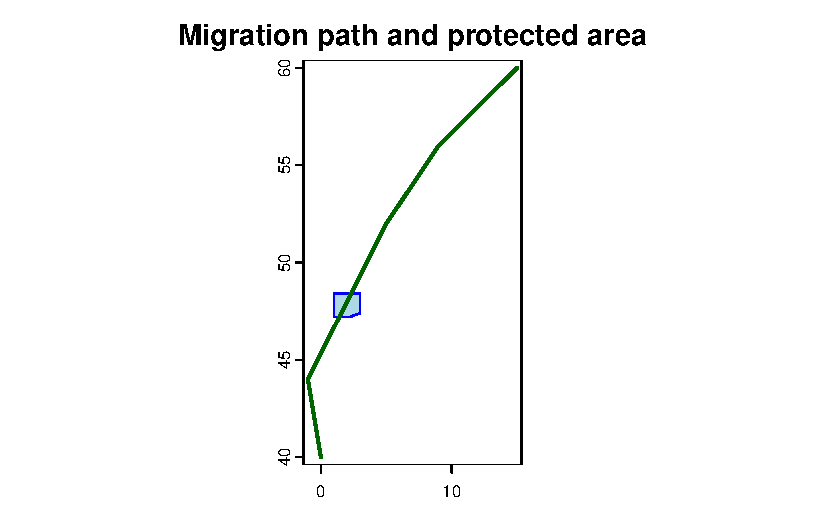
\includegraphics[keepaspectratio]{page_SDM.2_SpatialDataR_files/figure-pdf/unnamed-chunk-8-1.pdf}}

\begin{tcolorbox}[enhanced jigsaw, left=2mm, bottomtitle=1mm, colframe=quarto-callout-note-color-frame, title=\textcolor{quarto-callout-note-color}{\faInfo}\hspace{0.5em}{Insight: polygon closure}, breakable, coltitle=black, leftrule=.75mm, bottomrule=.15mm, arc=.35mm, toprule=.15mm, colback=white, toptitle=1mm, rightrule=.15mm, titlerule=0mm, opacityback=0, colbacktitle=quarto-callout-note-color!10!white, opacitybacktitle=0.6]

Polygons must have their first and last point identical to form a closed
shape --- otherwise they won't render as expected.

Always verify your coordinate order and closure when constructing
polygons manually.

\end{tcolorbox}

\section{1.3 Read Vector Data from
Files}\label{read-vector-data-from-files}

In real-world ecological and environmental projects, vector data are
rarely created manually. Instead, they are typically stored in spatial
file formats like:

\begin{itemize}
\tightlist
\item
  \textbf{Shapefile (\texttt{.shp})} -- the most widely used format for
  vector data; stores geometry and attributes across multiple sidecar
  files
\item
  \textbf{GeoJSON (\texttt{.geojson})} -- web-friendly and
  human-readable
\item
  \textbf{GPKG (GeoPackage)} -- a modern, single-file spatial format
\item
  \textbf{KML} -- often used for visualisation in tools like Google
  Earth
\end{itemize}

\begin{tcolorbox}[enhanced jigsaw, left=2mm, bottomtitle=1mm, colframe=quarto-callout-note-color-frame, title=\textcolor{quarto-callout-note-color}{\faInfo}\hspace{0.5em}{Insight: Common sources of vector-based biodiversity data}, breakable, coltitle=black, leftrule=.75mm, bottomrule=.15mm, arc=.35mm, toprule=.15mm, colback=white, toptitle=1mm, rightrule=.15mm, titlerule=0mm, opacityback=0, colbacktitle=quarto-callout-note-color!10!white, opacitybacktitle=0.6]

We live in an era of \textbf{big data}, where \textbf{biodiversity
datasets} are increasingly available in digital format and at
\textbf{global scale}. These data can come from:

\begin{itemize}
\tightlist
\item
  Standardised monitoring schemes\\
\item
  Citizen science platforms\\
\item
  Expert-drawn range maps
\end{itemize}

Each data source has its own strengths and limitations. In this
workshop, we'll explore different types of spatial biodiversity data and
how to load and visualise them in R.

In this session, we focus on basic description of data types, more on
the species and environmental data will be described in after sections
of the workshop.

\end{tcolorbox}

\begin{center}\rule{0.5\linewidth}{0.5pt}\end{center}

\subsection{\texorpdfstring{Base maps as an example of polygons (using
\texttt{rnaturalearth})}{Base maps as an example of polygons (using rnaturalearth)}}\label{base-maps-as-an-example-of-polygons-using-rnaturalearth}

To provide geographic context, we often need base maps of countries,
continents, or regions. The
\texttt{rnaturalearth}(https://github.com/ropensci/rnaturalearth)
package provides an excellent interface to the Natural Earth datasets.

Below is the code used to create spatial objects for the \textbf{UK} and
the \textbf{East Wales} region.\\
These have already been prepared in advance and saved to disk to speed
up the workshop.

\begin{tcolorbox}[enhanced jigsaw, left=2mm, bottomtitle=1mm, colframe=quarto-callout-note-color-frame, title=\textcolor{quarto-callout-note-color}{\faInfo}\hspace{0.5em}{Code to generate the spatial layers (already done in data preparation)}, breakable, coltitle=black, leftrule=.75mm, bottomrule=.15mm, arc=.35mm, toprule=.15mm, colback=white, toptitle=1mm, rightrule=.15mm, titlerule=0mm, opacityback=0, colbacktitle=quarto-callout-note-color!10!white, opacitybacktitle=0.6]

\begin{Shaded}
\begin{Highlighting}[]
\FunctionTok{library}\NormalTok{(rnaturalearth)}
\FunctionTok{library}\NormalTok{(sf)}

\CommentTok{\# Load country and region maps}
\NormalTok{World\_sf }\OtherTok{\textless{}{-}} \FunctionTok{ne\_countries}\NormalTok{(}\AttributeTok{scale =} \StringTok{"medium"}\NormalTok{, }\AttributeTok{returnclass =} \StringTok{"sf"}\NormalTok{)}
\NormalTok{UK\_sf }\OtherTok{\textless{}{-}} \FunctionTok{ne\_countries}\NormalTok{(}\AttributeTok{scale =} \StringTok{"medium"}\NormalTok{, }\AttributeTok{country =} \StringTok{"United Kingdom"}\NormalTok{, }\AttributeTok{returnclass =} \StringTok{"sf"}\NormalTok{)}
\NormalTok{UK\_admin\_sf }\OtherTok{\textless{}{-}} \FunctionTok{ne\_states}\NormalTok{(}\AttributeTok{country =} \StringTok{"United Kingdom"}\NormalTok{, }\AttributeTok{returnclass =} \StringTok{"sf"}\NormalTok{)}

\CommentTok{\# Subset to East Wales}
\NormalTok{WalesEast\_admin\_sf }\OtherTok{\textless{}{-}}\NormalTok{ UK\_admin\_sf[UK\_admin\_sf}\SpecialCharTok{$}\NormalTok{region }\SpecialCharTok{==} \StringTok{"East Wales"}\NormalTok{, ]}
\end{Highlighting}
\end{Shaded}

These steps are included in the data preparation file:\\
👉 \href{page_SDM.1_DataPreparation.qmd}{View full data preparation
script}

\end{tcolorbox}

\subsubsection{Visualise East Wales}\label{visualise-east-wales}

\begin{Shaded}
\begin{Highlighting}[]
\CommentTok{\# Load saved spatial objects}
\FunctionTok{library}\NormalTok{(ggplot2)}
\FunctionTok{library}\NormalTok{(sf)}

\CommentTok{\# Plot East Wales over the UK map}
\FunctionTok{ggplot}\NormalTok{() }\SpecialCharTok{+}
  \FunctionTok{geom\_sf}\NormalTok{(}\AttributeTok{data =}\NormalTok{ UK\_sf, }\AttributeTok{fill =} \StringTok{"grey90"}\NormalTok{, }\AttributeTok{color =} \StringTok{"black"}\NormalTok{) }\SpecialCharTok{+}
  \FunctionTok{geom\_sf}\NormalTok{(}\AttributeTok{data =}\NormalTok{ WalesEast\_admin\_sf, }\AttributeTok{fill =} \StringTok{"steelblue"}\NormalTok{, }\AttributeTok{color =} \StringTok{"darkblue"}\NormalTok{, }\AttributeTok{size =} \FloatTok{0.8}\NormalTok{) }\SpecialCharTok{+}
  \FunctionTok{labs}\NormalTok{(}
    \AttributeTok{title =} \StringTok{"East Wales within the United Kingdom"}
\NormalTok{  ) }\SpecialCharTok{+}
  \FunctionTok{theme\_minimal}\NormalTok{()}
\end{Highlighting}
\end{Shaded}

\begin{center}
\pandocbounded{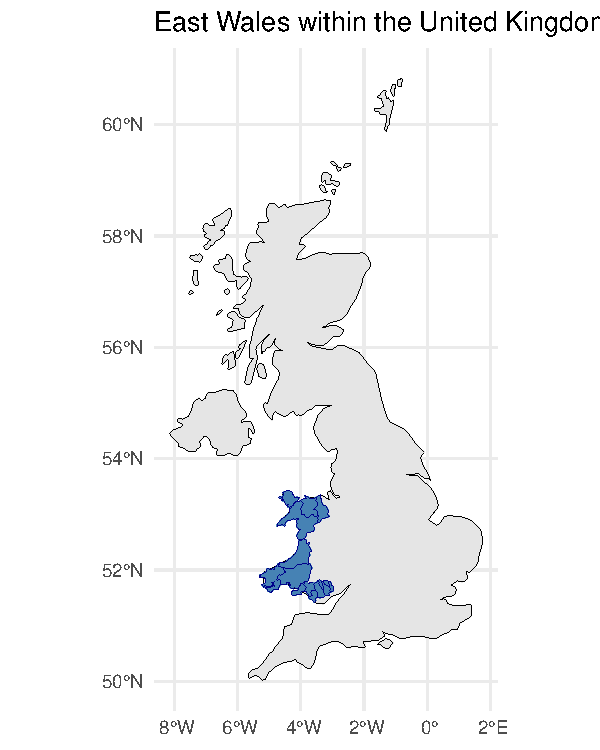
\includegraphics[keepaspectratio]{page_SDM.2_SpatialDataR_files/figure-pdf/plot-east-wales-1.pdf}}
\end{center}

\begin{tcolorbox}[enhanced jigsaw, left=2mm, bottomtitle=1mm, colframe=quarto-callout-note-color-frame, title=\textcolor{quarto-callout-note-color}{\faInfo}\hspace{0.5em}{Understanding spatial data structures in R}, breakable, coltitle=black, leftrule=.75mm, bottomrule=.15mm, arc=.35mm, toprule=.15mm, colback=white, toptitle=1mm, rightrule=.15mm, titlerule=0mm, opacityback=0, colbacktitle=quarto-callout-note-color!10!white, opacitybacktitle=0.6]

Familiarise yourself with the structure of \texttt{sp} and \texttt{sf}
spatial data formats. In this workshop, we use modern packages like
\texttt{sf} and \texttt{terra}, which follow the \textbf{Simple
Features} standard for spatial vector data.

Use the functions \texttt{crs()} (from \textbf{terra}) or
\texttt{st\_crs()} (from \textbf{sf}) to inspect and manipulate
\textbf{coordinate reference systems (CRS)}. These determine how
geometries relate to real-world locations and are essential when
combining spatial layers.

To learn more, check the
\href{https://r-spatial.github.io/sf/articles/sf1.html}{Simple Features
vignette} or run:

\begin{Shaded}
\begin{Highlighting}[]
\FunctionTok{vignette}\NormalTok{(}\StringTok{"sf1"}\NormalTok{, }\AttributeTok{package =} \StringTok{"sf"}\NormalTok{)}
\end{Highlighting}
\end{Shaded}

The website\href{https://rspatial.org/}{rspatial.org}, developed by a
team of researchers led by Robert J. Hijmans, is an excellent resource
for learning more about spatial data analysis and modeling in R.

\end{tcolorbox}

\begin{tcolorbox}[enhanced jigsaw, left=2mm, bottomtitle=1mm, colframe=quarto-callout-note-color-frame, title=\textcolor{quarto-callout-note-color}{\faInfo}\hspace{0.5em}{Key spatial vector workflow skills}, breakable, coltitle=black, leftrule=.75mm, bottomrule=.15mm, arc=.35mm, toprule=.15mm, colback=white, toptitle=1mm, rightrule=.15mm, titlerule=0mm, opacityback=0, colbacktitle=quarto-callout-note-color!10!white, opacitybacktitle=0.6]

\begin{itemize}
\tightlist
\item
  Use \texttt{terra::vect()} to read shapefiles (e.g., IUCN range
  maps)\\
\item
  Use \texttt{rnaturalearth::ne\_countries()} to get base maps of
  countries or continents\\
\item
  Combine both to map species ranges in a geographic context\\
\item
  Always check file format, coordinate reference system (CRS), and
  attribute content when working with real-world spatial data\\
\end{itemize}

\end{tcolorbox}

\section{2. Raster Data in R}\label{raster-data-in-r}

Raster datasets often come in file formats such as:

\begin{itemize}
\item
  \textbf{.tif (GeoTIFF)} --- the most widely used raster format
\item
  \textbf{.grd} --- often used in older R workflows
\item
  \textbf{.nc (NetCDF)} --- commonly used in climate science
\end{itemize}

We use the \texttt{terra} package to read and manipulate raster data in
R. From this package, the function \texttt{terra::rast()} is used to
create or read \texttt{SpatRaster} objects (the primary raster data
class in \texttt{terra}).

\begin{Shaded}
\begin{Highlighting}[]
\CommentTok{\# Create a raster from scratch}
\NormalTok{raster\_1 }\OtherTok{\textless{}{-}}\NormalTok{ terra}\SpecialCharTok{::}\FunctionTok{rast}\NormalTok{(}\AttributeTok{ncol =} \DecValTok{50}\NormalTok{, }\AttributeTok{nrow =} \DecValTok{50}\NormalTok{, }\AttributeTok{xmin =} \DecValTok{0}\NormalTok{, }\AttributeTok{xmax =} \DecValTok{50}\NormalTok{,  }\AttributeTok{ymin =} \DecValTok{0}\NormalTok{, }\AttributeTok{ymax =} \DecValTok{50}\NormalTok{)}
\end{Highlighting}
\end{Shaded}

We can access the attributes of each raster cell by using the function
\texttt{terra::values()}. Obviously, there are no values yet in the
\texttt{SpatRaster} object and thus we assign some, generating random
numbers with \texttt{rnorm()}:

\begin{Shaded}
\begin{Highlighting}[]
\CommentTok{\# Check the summary stats of the values in raster\_1:}
\FunctionTok{summary}\NormalTok{(terra}\SpecialCharTok{::}\FunctionTok{values}\NormalTok{(raster\_1))}
\end{Highlighting}
\end{Shaded}

\begin{verbatim}
Warning: [readValues] raster has no values
\end{verbatim}

\begin{verbatim}
     lyr.1     
 Min.   : NA   
 1st Qu.: NA   
 Median : NA   
 Mean   :NaN   
 3rd Qu.: NA   
 Max.   : NA   
 NA's   :2500  
\end{verbatim}

\begin{Shaded}
\begin{Highlighting}[]
\CommentTok{\# Assign values (randomly drawn from normal distribution) to the SpatRaster object:}
\NormalTok{terra}\SpecialCharTok{::}\FunctionTok{values}\NormalTok{(raster\_1) }\OtherTok{\textless{}{-}} \FunctionTok{rnorm}\NormalTok{(}\FunctionTok{ncell}\NormalTok{(raster\_1))}

\CommentTok{\# plot the raster}
\FunctionTok{plot}\NormalTok{(raster\_1)}
\end{Highlighting}
\end{Shaded}

\begin{center}
\pandocbounded{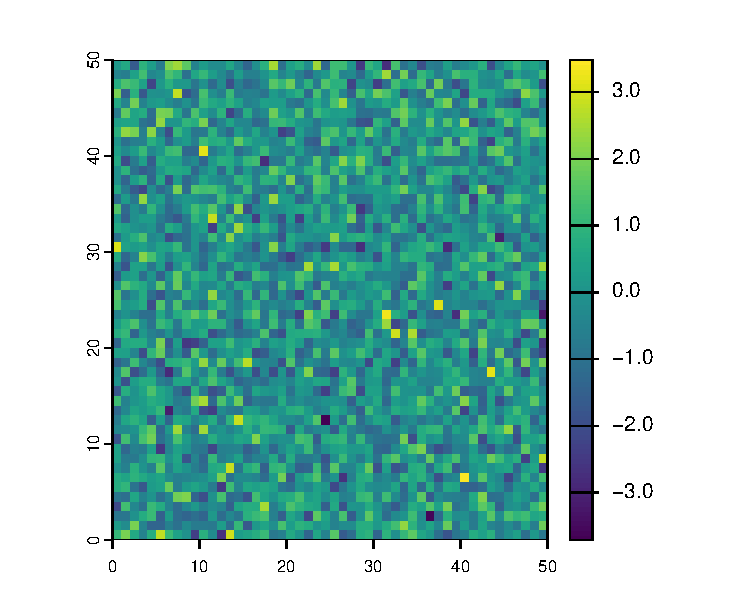
\includegraphics[keepaspectratio]{page_SDM.2_SpatialDataR_files/figure-pdf/unnamed-chunk-12-1.pdf}}
\end{center}

Raster resolution determines the spatial grain of your data --- the size
of each pixel on the ground. Higher resolution (e.g., 10m) provides more
detail, but is computationally heavier.

This concept of spatial scale is crucial in ecology. Analyses done at
fine scales may yield different insights than those at coarse scales.

To demonstrate this, we aggregate the raster to a coarser resolution.
With multiple raster objects at hand, combine layers into a multi-layer
\texttt{SpatRaster} object using the \texttt{terra::rast()} function to
concatenate the layers.

\begin{Shaded}
\begin{Highlighting}[]
\CommentTok{\# Aggregate the raster to a coarser resolution (2x2)}
\NormalTok{raster\_2 }\OtherTok{\textless{}{-}} \FunctionTok{aggregate}\NormalTok{(raster\_1, }\AttributeTok{fact =} \DecValTok{2}\NormalTok{, }\AttributeTok{fun =}\NormalTok{ mean)}

\CommentTok{\# Match raster\_2 (coarse) to raster\_1 (fine resolution)}
\NormalTok{raster\_2\_resamp }\OtherTok{\textless{}{-}} \FunctionTok{resample}\NormalTok{(raster\_2, raster\_1, }\AttributeTok{method =} \StringTok{"bilinear"}\NormalTok{)}

\CommentTok{\# Create multi{-}layer raster object}
\NormalTok{raster\_multi }\OtherTok{\textless{}{-}} \FunctionTok{c}\NormalTok{(raster\_1, raster\_2\_resamp)}

\CommentTok{\# Assign layer names}
\FunctionTok{names}\NormalTok{(raster\_multi) }\OtherTok{\textless{}{-}} \FunctionTok{c}\NormalTok{(}\StringTok{"Fine resolution"}\NormalTok{, }\StringTok{"Coarse resolution"}\NormalTok{)}

\CommentTok{\# Plot the raster layers}
\FunctionTok{plot}\NormalTok{(raster\_multi)}
\end{Highlighting}
\end{Shaded}

\begin{center}
\pandocbounded{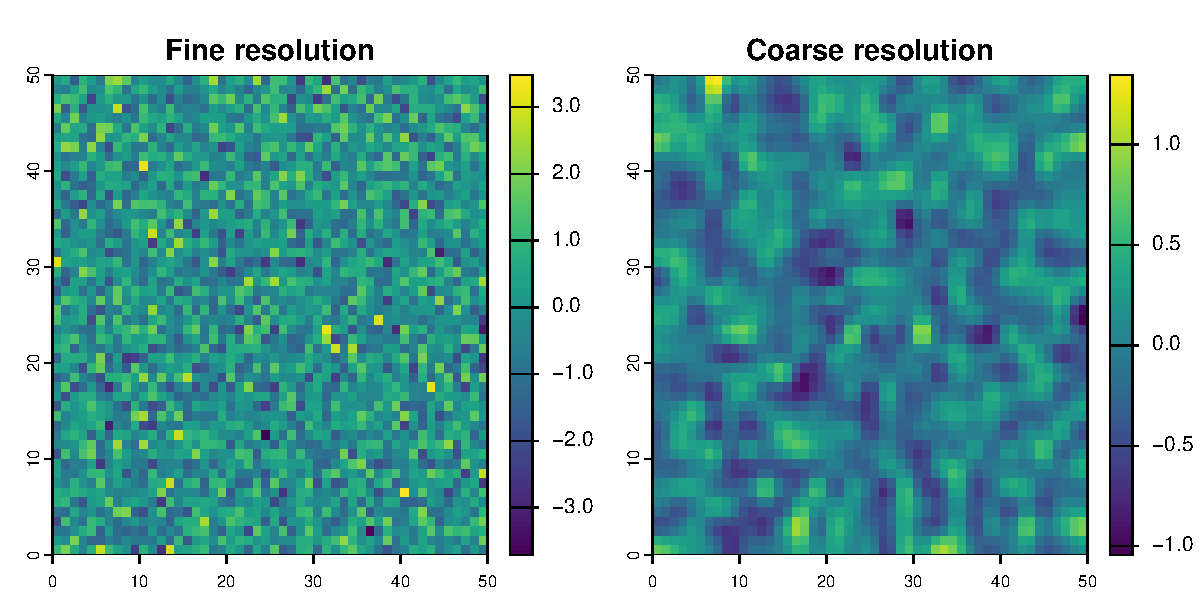
\includegraphics[keepaspectratio]{page_SDM.2_SpatialDataR_files/figure-pdf/unnamed-chunk-13-1.pdf}}
\end{center}

\section{2.1 Read raster data from
files}\label{read-raster-data-from-files}

In ecological and environmental research, raster data are commonly used
to represent \textbf{continuous environmental variables} like climate,
elevation, or land cover.

One widely used dataset is the \textbf{WorldClim v2.1 Bioclimatic
Variables}, which provides global climate data at multiple resolutions.
You can explore the available variables
\href{https://www.worldclim.org/data/bioclim.html}{here}. To download
and use these data in R, this can be efficiently done with the
\texttt{geodata} package (part of the \texttt{rspatial} site developed
by the \href{https://rspatial.org/}{rspatial.org} group led by Robert J.
Hijmans).

\subsection{Code to download WorldClim 2.1 bioclimatic variables
(already done in data
preparation)}\label{code-to-download-worldclim-2.1-bioclimatic-variables-already-done-in-data-preparation}

\begin{Shaded}
\begin{Highlighting}[]
\FunctionTok{library}\NormalTok{(geodata)}

\CommentTok{\# download WorldClim 2.1 bioclimatic variables (10{-}minute resolution, this returns a SpatRaster with 19 layers, bio1 to bio19)}
\NormalTok{Clim\_extant }\OtherTok{\textless{}{-}}\NormalTok{ geodata}\SpecialCharTok{::}\FunctionTok{worldclim\_global}\NormalTok{(}\AttributeTok{var =} \StringTok{"bio"}\NormalTok{, }\AttributeTok{res =} \DecValTok{5}\NormalTok{, }\AttributeTok{path =} \StringTok{"data/"}\NormalTok{)}

\CommentTok{\# Crop climate to UK}
\NormalTok{Clim\_UK }\OtherTok{\textless{}{-}}\NormalTok{ terra}\SpecialCharTok{::}\FunctionTok{crop}\NormalTok{(Clim\_extant, UK\_sf)}
\end{Highlighting}
\end{Shaded}

These steps are included in the data preparation file:\\
👉 \href{page_SDM.1_DataPreparation}{View full data preparation script}

We can now extract the focal data of interest, here we crop the mean
annual precipitation (bio12) data to the spatial extent of the UK.

\begin{Shaded}
\begin{Highlighting}[]
\CommentTok{\#| fig{-}width: 4}
\CommentTok{\#| fig{-}height: 5}
\CommentTok{\#| fig{-}align: left}

\CommentTok{\# Extract Bioclim variable 12: annual precipitation}
\NormalTok{precip\_UK }\OtherTok{\textless{}{-}}\NormalTok{ Clim\_UK[[}\DecValTok{12}\NormalTok{]]  }\CommentTok{\# bio12: annual precipitation in mm}

\CommentTok{\# Plot the precipitation map}
\NormalTok{terra}\SpecialCharTok{::}\FunctionTok{plot}\NormalTok{(precip\_UK, }\AttributeTok{main =} \StringTok{"Mean annual precipitation (bio12) {-} UK"}\NormalTok{)}
\end{Highlighting}
\end{Shaded}

\pandocbounded{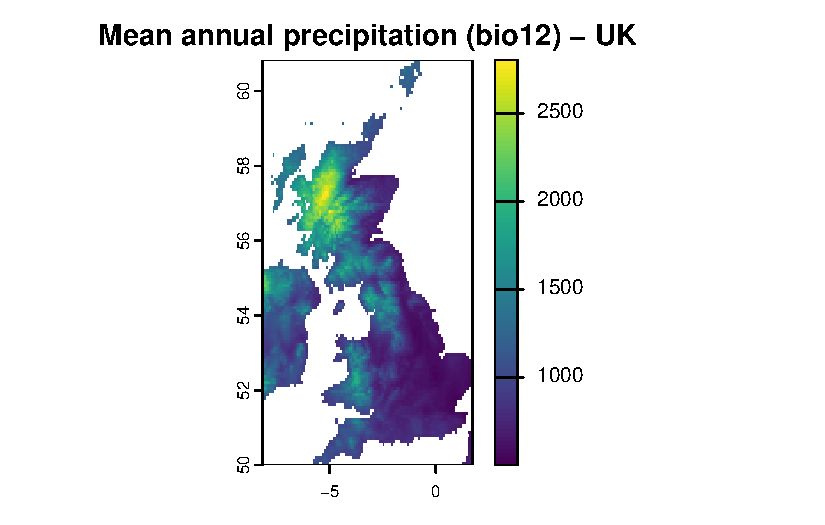
\includegraphics[keepaspectratio]{page_SDM.2_SpatialDataR_files/figure-pdf/unnamed-chunk-15-1.pdf}}

\begin{tcolorbox}[enhanced jigsaw, left=2mm, bottomtitle=1mm, colframe=quarto-callout-tip-color-frame, title=\textcolor{quarto-callout-tip-color}{\faLightbulb}\hspace{0.5em}{Tip: Coordinate systems must match}, breakable, coltitle=black, leftrule=.75mm, bottomrule=.15mm, arc=.35mm, toprule=.15mm, colback=white, toptitle=1mm, rightrule=.15mm, titlerule=0mm, opacityback=0, colbacktitle=quarto-callout-tip-color!10!white, opacitybacktitle=0.6]

When working with raster and vector data together (e.g., cropping or
masking), ensure both objects use the \textbf{same CRS}. Use
\texttt{terra::project()} to reproject if needed.

\end{tcolorbox}

\section{2.2 Manipulate raster data}\label{manipulate-raster-data}

\paragraph{Reproject raster data}\label{reproject-raster-data}

\begin{Shaded}
\begin{Highlighting}[]
\CommentTok{\# Reproject raster to a different CRS (e.g. British National Grid EPSG:27700)}
\NormalTok{precip\_UK\_proj }\OtherTok{\textless{}{-}}\NormalTok{ terra}\SpecialCharTok{::}\FunctionTok{project}\NormalTok{(precip\_UK, }\StringTok{"EPSG:27700"}\NormalTok{)}

\NormalTok{terra}\SpecialCharTok{::}\FunctionTok{plot}\NormalTok{(precip\_UK\_proj, }\AttributeTok{main =} \StringTok{"Precipitation (Reprojected)"}\NormalTok{)}
\end{Highlighting}
\end{Shaded}

\pandocbounded{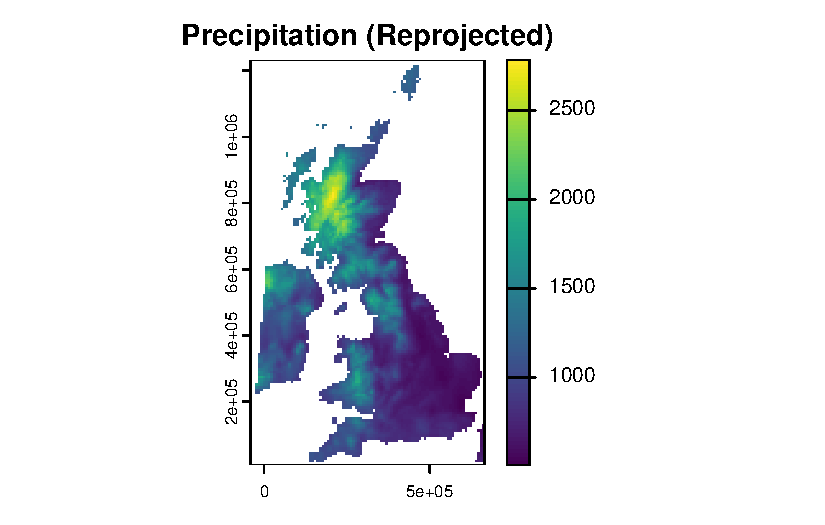
\includegraphics[keepaspectratio]{page_SDM.2_SpatialDataR_files/figure-pdf/unnamed-chunk-16-1.pdf}}

\paragraph{Raster math / algebra}\label{raster-math-algebra}

\begin{Shaded}
\begin{Highlighting}[]
\CommentTok{\#| fig{-}width: 4}
\CommentTok{\#| fig{-}height: 5}
\CommentTok{\#| fig{-}align: left}

\CommentTok{\# Math / algebra example: Convert mm to cm for precipitation}
\NormalTok{precip\_cm }\OtherTok{\textless{}{-}}\NormalTok{ precip\_UK }\SpecialCharTok{/} \DecValTok{10}

\CommentTok{\# Difference between original and converted}
\NormalTok{terra}\SpecialCharTok{::}\FunctionTok{plot}\NormalTok{(precip\_cm }\SpecialCharTok{{-}}\NormalTok{ precip\_UK, }\AttributeTok{main =} \StringTok{"Difference after unit conversion"}\NormalTok{)}
\end{Highlighting}
\end{Shaded}

\pandocbounded{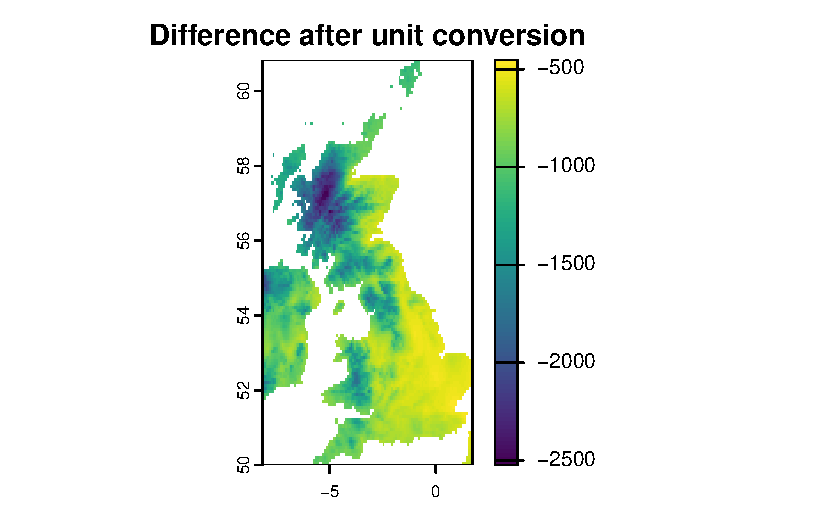
\includegraphics[keepaspectratio]{page_SDM.2_SpatialDataR_files/figure-pdf/unnamed-chunk-17-1.pdf}}

\begin{Shaded}
\begin{Highlighting}[]
\CommentTok{\# Apply mean filter with 3x3 window}
\NormalTok{focal\_mean }\OtherTok{\textless{}{-}}\NormalTok{ terra}\SpecialCharTok{::}\FunctionTok{focal}\NormalTok{(precip\_UK, }\AttributeTok{w =} \FunctionTok{matrix}\NormalTok{(}\DecValTok{1}\NormalTok{, }\DecValTok{3}\NormalTok{, }\DecValTok{3}\NormalTok{), }\AttributeTok{fun =}\NormalTok{ mean, }\AttributeTok{na.policy =} \StringTok{"omit"}\NormalTok{)}

\NormalTok{terra}\SpecialCharTok{::}\FunctionTok{plot}\NormalTok{(focal\_mean, }\AttributeTok{main =} \StringTok{"Smoothed Precipitation (3x3 mean)"}\NormalTok{)}
\end{Highlighting}
\end{Shaded}

\pandocbounded{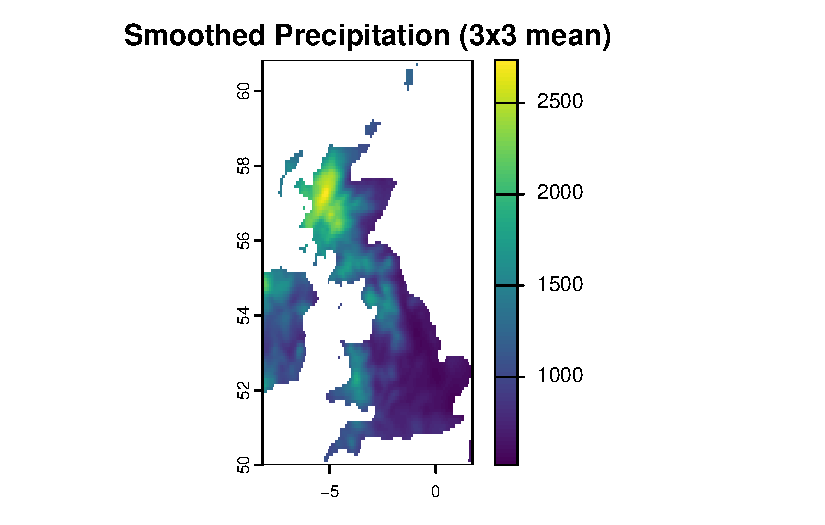
\includegraphics[keepaspectratio]{page_SDM.2_SpatialDataR_files/figure-pdf/unnamed-chunk-17-2.pdf}}

\paragraph{Zonal statistics}\label{zonal-statistics}

Summarising raster data over polygonal spatial units is a common task in
ecological and environmental analysis (and the broader field of applied
data science). This is known as zonal statistics. For example, we can
compute and visualise mean annual precipitation across UK administrative
zones using the \texttt{terra} and \texttt{ggplot2} packages:

\begin{Shaded}
\begin{Highlighting}[]
\CommentTok{\#| fig{-}width: 4}
\CommentTok{\#| fig{-}height: 5}
\CommentTok{\#| fig{-}align: left}

\CommentTok{\# Add an ID column to UK\_admin\_sf (to explicitly match IDs between zonal\_means and UK\_admin\_sf below)}
\NormalTok{UK\_admin\_sf}\SpecialCharTok{$}\NormalTok{admin\_id }\OtherTok{\textless{}{-}} \DecValTok{1}\SpecialCharTok{:}\FunctionTok{nrow}\NormalTok{(UK\_admin\_sf)}

\CommentTok{\# Convert UK\_admin\_sf to SpatVector}
\NormalTok{zones\_vect }\OtherTok{\textless{}{-}}\NormalTok{ terra}\SpecialCharTok{::}\FunctionTok{vect}\NormalTok{(UK\_admin\_sf)}

\CommentTok{\# Compute mean precipitation by zone}
\NormalTok{zonal\_means }\OtherTok{\textless{}{-}}\NormalTok{ terra}\SpecialCharTok{::}\FunctionTok{extract}\NormalTok{(precip\_UK, zones\_vect, }\AttributeTok{fun =}\NormalTok{ mean, }\AttributeTok{na.rm =} \ConstantTok{TRUE}\NormalTok{, }\AttributeTok{ID =} \ConstantTok{TRUE}\NormalTok{)}

\CommentTok{\# Preview output}
\FunctionTok{head}\NormalTok{(zonal\_means)}
\end{Highlighting}
\end{Shaded}

\begin{verbatim}
  ID   bio_12
1  1 1504.444
2  2 1716.789
3  3 1312.486
4  4 1131.222
5  5 1029.231
6  6 1376.529
\end{verbatim}

\begin{Shaded}
\begin{Highlighting}[]
\CommentTok{\# Replace NA values with 0 for demonstration purposes}
\CommentTok{\# !Note: This should be done cautiously — replacing NA may not be appropriate depending on your analysis.}
\NormalTok{precip\_no\_na }\OtherTok{\textless{}{-}}\NormalTok{ terra}\SpecialCharTok{::}\FunctionTok{classify}\NormalTok{(precip\_UK, }\FunctionTok{cbind}\NormalTok{(}\ConstantTok{NA}\NormalTok{, }\DecValTok{0}\NormalTok{))}

\CommentTok{\# Merge zonal means (bio12 = mean annual precipitation) back to the spatial data (ensure correct ID match)}
\NormalTok{UK\_admin\_sf}\SpecialCharTok{$}\NormalTok{mean\_precip\_mm }\OtherTok{\textless{}{-}}\NormalTok{ zonal\_means}\SpecialCharTok{$}\NormalTok{bio\_12[}\FunctionTok{match}\NormalTok{(UK\_admin\_sf}\SpecialCharTok{$}\NormalTok{admin\_id, zonal\_means}\SpecialCharTok{$}\NormalTok{ID)]}

\CommentTok{\# Plot the map of mean precipitation by zone}
\FunctionTok{ggplot}\NormalTok{(UK\_admin\_sf) }\SpecialCharTok{+}
  \FunctionTok{geom\_sf}\NormalTok{(}\FunctionTok{aes}\NormalTok{(}\AttributeTok{fill =}\NormalTok{ mean\_precip\_mm), }\AttributeTok{color =} \StringTok{"white"}\NormalTok{) }\SpecialCharTok{+}
  \FunctionTok{scale\_fill\_viridis\_c}\NormalTok{(}\AttributeTok{name =} \StringTok{"Annual Precipitation (mm)"}\NormalTok{, }\AttributeTok{na.value =} \StringTok{"grey90"}\NormalTok{) }\SpecialCharTok{+}
  \FunctionTok{labs}\NormalTok{(}
    \AttributeTok{title =} \StringTok{"Annual precipitation by UK administrative zone"}\NormalTok{,}
    \AttributeTok{caption =} \StringTok{"Data source: WorldClim 2.1 + Natural Earth"}
\NormalTok{  ) }\SpecialCharTok{+}
  \FunctionTok{theme\_minimal}\NormalTok{()}
\end{Highlighting}
\end{Shaded}

\pandocbounded{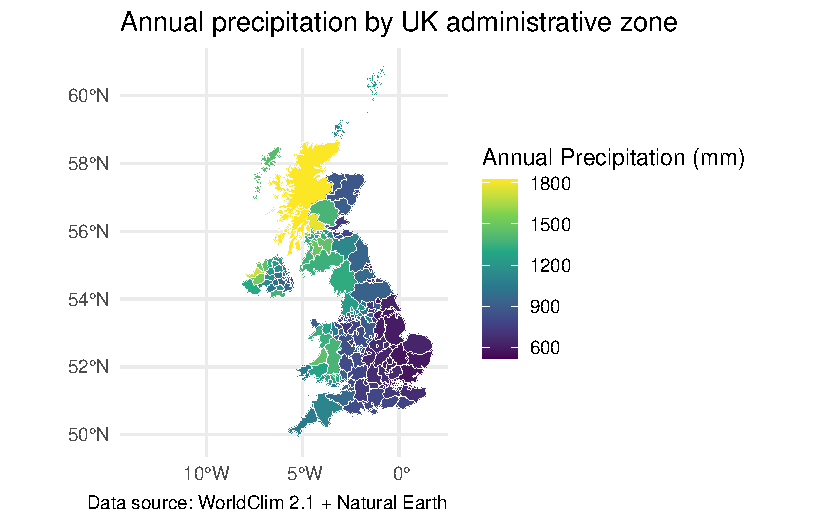
\includegraphics[keepaspectratio]{page_SDM.2_SpatialDataR_files/figure-pdf/unnamed-chunk-18-1.pdf}}

\section{2.3 Extract Raster Values}\label{extract-raster-values}

Extracting raster values at specific locations is a key step in many
ecological and environmental workflows, particularly in species
distribution modelling. This process allows us to link spatially
continuous variables---such as climate or elevation---to discrete
observation points, like species occurrence records. In this section, we
demonstrate how to extract raster values using the \texttt{terra}
package, both for point locations and across multiple raster layers.

\begin{Shaded}
\begin{Highlighting}[]
\CommentTok{\# Set seed for reproducibility}
\FunctionTok{set.seed}\NormalTok{(}\DecValTok{1}\NormalTok{)}

\CommentTok{\# Convert UK\_sf object (an sf object) into a SpatVector object}
\NormalTok{UK\_vect }\OtherTok{\textless{}{-}}\NormalTok{ terra}\SpecialCharTok{::}\FunctionTok{vect}\NormalTok{(UK\_sf)}

\CommentTok{\# Simulate some (arbitrary) species occurrence points within the UK}
\NormalTok{occ\_points }\OtherTok{\textless{}{-}}\NormalTok{ terra}\SpecialCharTok{::}\FunctionTok{spatSample}\NormalTok{(UK\_vect[,}\DecValTok{1}\NormalTok{], }\AttributeTok{size =} \DecValTok{100}\NormalTok{, }\AttributeTok{method =} \StringTok{"random"}\NormalTok{)}

\CommentTok{\# Extract raster values at these point locations}
\NormalTok{occ\_precip }\OtherTok{\textless{}{-}}\NormalTok{ terra}\SpecialCharTok{::}\FunctionTok{extract}\NormalTok{(precip\_UK, occ\_points)}

\CommentTok{\# Combine coordinates and extracted values}
\NormalTok{occ\_df }\OtherTok{\textless{}{-}} \FunctionTok{cbind}\NormalTok{(}\FunctionTok{as.data.frame}\NormalTok{(occ\_points), }\AttributeTok{precip\_mm =}\NormalTok{ occ\_precip[,}\DecValTok{2}\NormalTok{])}

\FunctionTok{head}\NormalTok{(occ\_df)}
\end{Highlighting}
\end{Shaded}

\begin{verbatim}
       featurecla precip_mm
1 Admin-0 country       813
2 Admin-0 country       897
3 Admin-0 country       599
4 Admin-0 country       857
5 Admin-0 country       577
6 Admin-0 country      1472
\end{verbatim}

\begin{Shaded}
\begin{Highlighting}[]
\CommentTok{\# Extract all 19 bioclim variables (multiple raster layers) for each point}
\NormalTok{clim\_data\_vals }\OtherTok{\textless{}{-}}\NormalTok{ terra}\SpecialCharTok{::}\FunctionTok{extract}\NormalTok{(Clim\_UK, occ\_points)}

\CommentTok{\# Combine with species occurrence coordinates}
\NormalTok{clim\_data\_df }\OtherTok{\textless{}{-}} \FunctionTok{cbind}\NormalTok{(}\FunctionTok{as.data.frame}\NormalTok{(occ\_points), clim\_data\_vals[,}\SpecialCharTok{{-}}\DecValTok{1}\NormalTok{])  }\CommentTok{\# Remove ID column}

\FunctionTok{head}\NormalTok{(clim\_data\_df)}
\end{Highlighting}
\end{Shaded}

\begin{verbatim}
       featurecla    bio_1    bio_2    bio_3    bio_4    bio_5     bio_6
1 Admin-0 country 7.281042 7.019583 38.77366 413.2269 17.42100 -0.683000
2 Admin-0 country 9.604292 7.539417 37.85608 463.8675 21.04300  1.127000
3 Admin-0 country 9.550167 8.080500 38.05275 486.4427 21.86000  0.625000
4 Admin-0 country 6.861417 7.221333 38.35219 432.1033 17.46600 -1.363000
5 Admin-0 country 9.800042 6.891583 34.70257 477.9860 21.01500  1.156000
6 Admin-0 country 8.965159 7.169326 39.33672 417.4897 19.32128  1.095745
     bio_7     bio_8     bio_9   bio_10   bio_11 bio_12 bio_13 bio_14   bio_15
1 18.10400  7.780500  8.499666 12.63950 2.659833    813     85     55 15.05392
2 19.91600  5.297667 13.855500 15.54483 4.369333    897    100     52 24.57603
3 21.23500 10.247167  5.786000 15.72250 3.987000    599     59     37 13.67015
4 18.82900  4.599000  8.310667 12.46333 1.977000    857     94     57 18.63359
5 19.85900  7.771833  5.868667 15.91117 4.354167    577     61     34 19.14082
6 18.22553  4.776773 12.928192 14.33546 4.185993   1472    171     84 25.41553
  bio_16 bio_17 bio_18 bio_19
1    240    172    190    208
2    298    168    175    267
3    172    127    144    148
4    260    174    186    233
5    174    112    158    141
6    483    259    285    463
\end{verbatim}

\begin{tcolorbox}[enhanced jigsaw, left=2mm, bottomtitle=1mm, colframe=quarto-callout-note-color-frame, title=\textcolor{quarto-callout-note-color}{\faInfo}\hspace{0.5em}{Exercises: Load and Inspect a Raster}, breakable, coltitle=black, leftrule=.75mm, bottomrule=.15mm, arc=.35mm, toprule=.15mm, colback=white, toptitle=1mm, rightrule=.15mm, titlerule=0mm, opacityback=0, colbacktitle=quarto-callout-note-color!10!white, opacitybacktitle=0.6]

\begin{enumerate}
\def\labelenumi{\arabic{enumi}.}
\item
  \textbf{Load and plot raster:}\\
  Load the raster file \texttt{bioclim\_01.tif} using the \texttt{terra}
  package. Plot the raster using a unique and appropriate color scale
  (e.g., \texttt{viridis}).
\item
  \textbf{Extract climate values at city locations:}\\
  Use coordinates of 10 cities in the UK and Italy (or any other
  countries you choose). Extract and compare the climate values (mean
  annual temperature, bio1) at these points.
\item
  \textbf{Calculate zonal means for countries:}\\
  Using polygon shapefiles of European countries or countries worldwide,
  calculate the zonal mean of bio1 (mean annual temperature) for each
  country. Visualize the result with a choropleth map.
\end{enumerate}

\end{tcolorbox}

\begin{tcolorbox}[enhanced jigsaw, left=2mm, bottomtitle=1mm, colframe=quarto-callout-note-color-frame, title=\textcolor{quarto-callout-note-color}{\faInfo}\hspace{0.5em}{Useful sources}, breakable, coltitle=black, leftrule=.75mm, bottomrule=.15mm, arc=.35mm, toprule=.15mm, colback=white, toptitle=1mm, rightrule=.15mm, titlerule=0mm, opacityback=0, colbacktitle=quarto-callout-note-color!10!white, opacitybacktitle=0.6]

Hijmans, R. J. (2023). \emph{rspatial.org: Spatial Data in R}.
\url{https://rspatial.org/}

Lovelace, R., Nowosad, J., \& Muenchow, J. (2023). \emph{Geocomputation
with R}. \url{https://geocompr.robinlovelace.net}

Pebesma, E. (2023). \emph{Simple Features for R: Standardized Support
for Spatial Vector Data}.
\url{https://r-spatial.github.io/sf/index.html}

Pebesma, E., \& Bivand, R. (2025). \emph{Spatial Data Science: With
Applications in R.} \url{https://r-spatial.org/book/}

\end{tcolorbox}


\backmatter


\end{document}
